\documentclass[12pt,fleqn]{article}
\setlength{\parindent}{0pt}
\usepackage{graphicx}
\usepackage{cancel}
\usepackage{listings}
\usepackage[latin5]{inputenc}
\usepackage{color}
\setlength{\parskip}{8pt}
\setlength{\parsep}{0pt}
\setlength{\headsep}{0pt}
\setlength{\topskip}{0pt}
\setlength{\topmargin}{0pt}
\setlength{\topsep}{0pt}
\setlength{\partopsep}{0pt}
\setlength{\mathindent}{0cm}
\usepackage{latexsym}
\usepackage{showkeys}
\renewcommand*\showkeyslabelformat[1]{(#1)}

\begin{document}
Ders 23 

Bu ders Laplace Transformlarinin son dersi, ayni zamanda, yeni bir girdi
fonksiyonunu gorecegiz -- birim vurus (unit impulse) fonksiyonlari. Vurus
nedir? Tokat atmaktan bahsetmiyoruz tabii; vurus, mesela bir objeye bir zaman
surecinde $f(t)$ kuvveti uyguladigimizi dusunelim, 

\[ f(t) \textit{ vurusu } = \int _{a}^{b}f(t)dt \]

Eger $f(t)$ sabit ise, 

\[ Vurus = F \cdot (b-a) \]

Guc derken nasil bir sistemden bahsediyoruz? Mesela

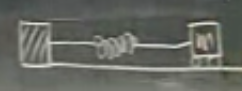
\includegraphics[height=2cm]{23_1.png}

Bu sisteme sagdan, belli bir sure bir guc uyguladigimizi dusunelim, $f(t)$
bu iste. 

Bu sistemin davranisini Laplace Transform ile cozmek icin kuvveti nasil
modellerim? Diyelim ki 

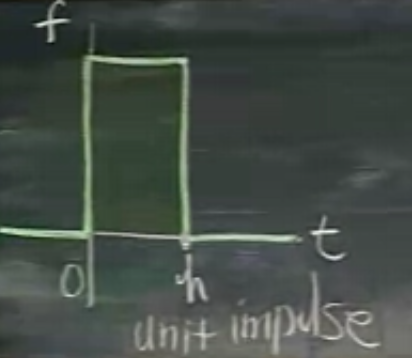
\includegraphics[height=3cm]{23_2.png}

0 aninda kuvvet uygulamasi basliyor, 0'dan 1'e cikiyoruz, $h$ kadar devam
ediyor, sonra sifira iniyor. 

















\end{document}
